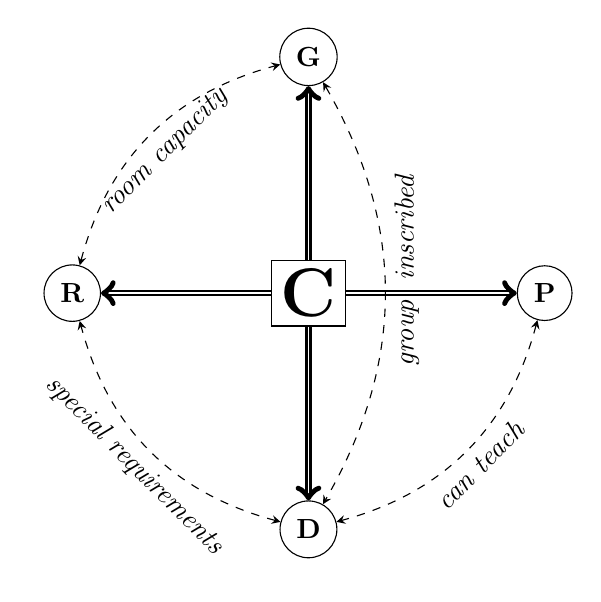
\begin{tikzpicture}
 
\edef\r{3cm}

\node[draw]         (C) at (0,  0) {\textbf{\Huge C}};
\node[draw, circle] (G) at (0, \r) {\textbf{G}};
\node[draw, circle] (P) at (\r, 0) {\textbf{P}};
\node[draw, circle] (D) at (0,-\r) {\textbf{D}};
\node[draw, circle] (R) at (-\r,0) {\textbf{R}};

\foreach \i in {(G),(P),(D),(R)}
 \draw[->, thick, double] (C) -- \i;

\def\data{ P/D/can teach
         , D/R/special requirements
         , R/G/room capacity
         , G/D/\quad~ group~~inscribed
         }

\foreach \i/\j/\k in \data
 \draw[<->, >=stealth, dashed] (\i) to[bend left
                                      ,edge node={node [sloped, below] {\emph{\k}}}]
                               (\j);


\end{tikzpicture}